\documentclass[11pt,oneside]{memoir}

\usepackage{schedule}

\title{Vinaya Class Schedule}
\author{The Bhikkhu Saṅgha}

\hypersetup{
  pdftitle={\thetitle},
  pdfauthor={\theauthor},
  pdfcopyright={Copyright (C) \the\year, \theauthor},
  pdfsubject={buddhism, vinaya},
  pdfkeywords={buddhism, vinaya},
  pdflicenseurl={https://creativecommons.org/licenses/by-nc-nd/4.0/},
  pdfcontacturl={https://vinaya-class.github.io/},
  pdflang={en},
}

\begin{document}

\thispagestyle{empty}

\vspace*{-10mm}
{\centering
  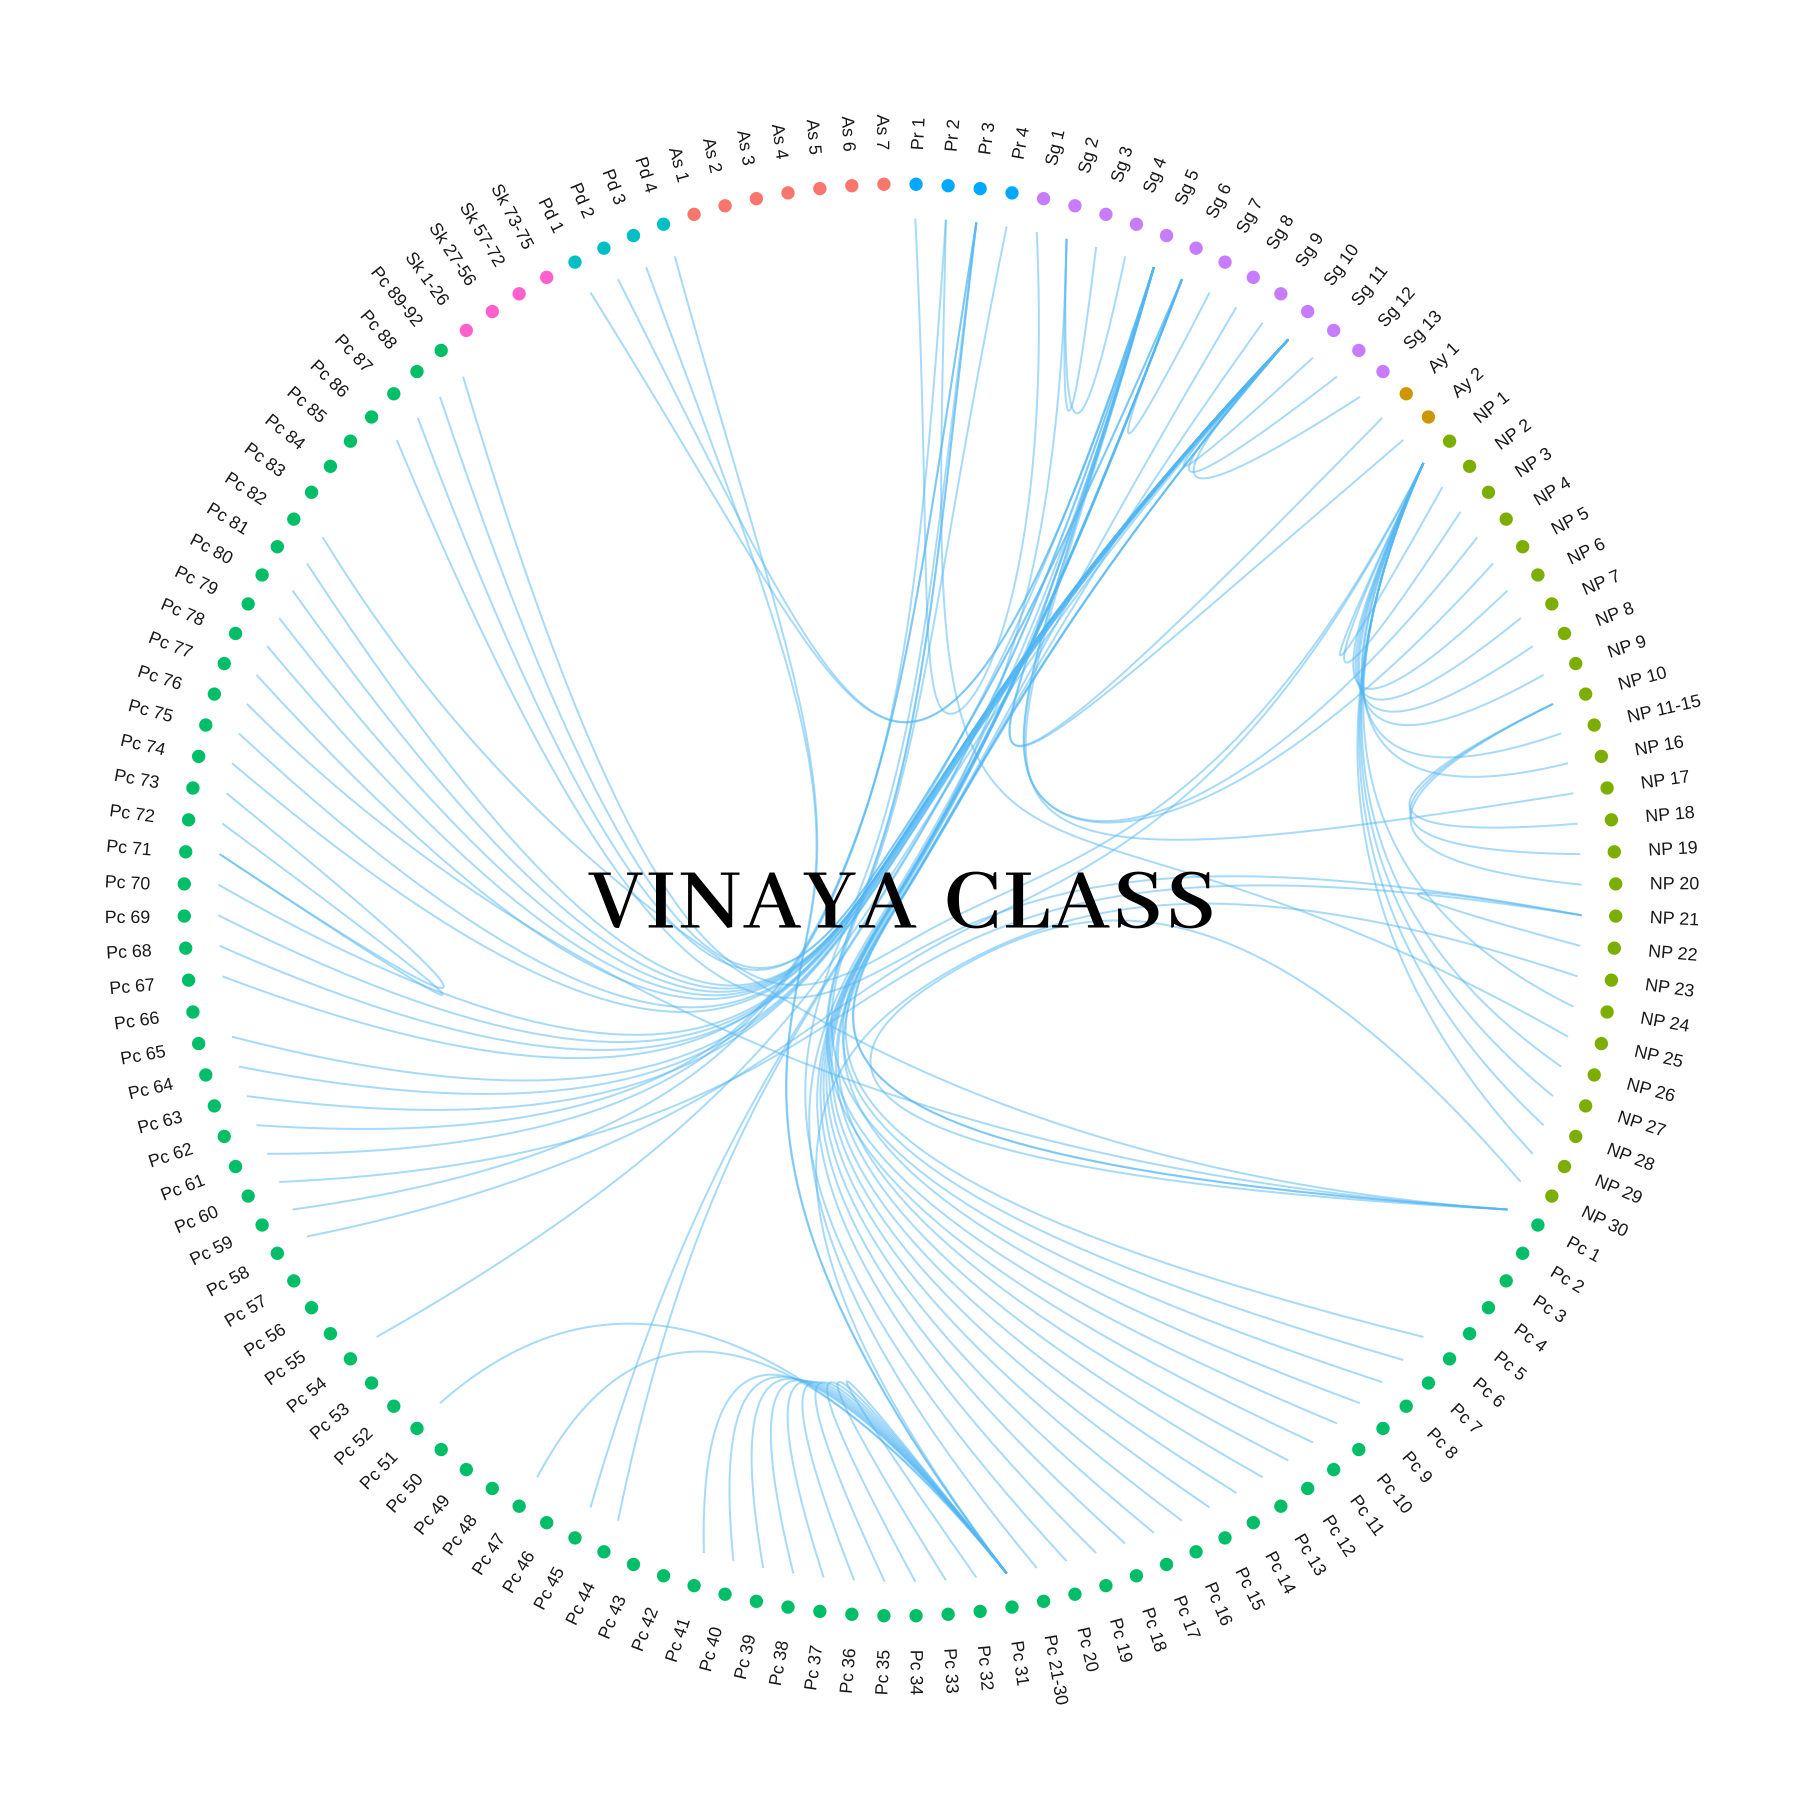
\includegraphics[width=100mm]{../../assets/vinaya-class-title/vinaya-class-title-300dpi.png}
\par}

\bigskip

\chapter{Class 1}

\centeringsectiontrue

{\centering
\sectionFmt{Introduction}

%\hspace*{22pt}
\numberbullet{1} Purpose and functional operation of the Vinaya\quad
\numberbullet{2} Overview of the rules\quad
\numberbullet{3} Reference books

\orig{} marks rules with recommended origin stories
\par}

\centeringsectionfalse
\numberedtopicstrue

\chapter{Class 2}

\begin{multicols}{2}

\section{Killing and harming}

\begin{description}
\item[Pr 3 \orig] Killing a human being or advocating death
\item[Pc 61 \orig] Killing an animal
\item[Pc 20] Pouring water containing living beings
\item[Pc 62] Using water containing living beings
\item[Pc 10] Digging soil
\item[Pc 11 \orig] Damaging living plants or seeds% p.324
\end{description}

\columnbreak

\section{Stealing}

\begin{description}
\item[Pr 2 \orig] Stealing
\item[NP 25 \orig] Snatching back robe% p.272
\item[Pc 59] Using cloth or bowl under shared ownership
\end{description}

\end{multicols}

\chapter{Class 3}

\begin{multicols}{2}

\section{Sexual conduct}

\begin{description}
\item[Pr 1 \orig] Sexual intercourse% p.4, p.43
\item[Sg 1 \orig] Intentional emission of semen% p.112
\end{description}

\section{Lustful conduct}

\begin{description}
\item[Sg 2 \orig] Lustful contact with a woman% p.121
\item[Sg 3 \orig] Speaking lewd words to a woman% p.132
\item[Sg 4 \orig] Praising sexual intercourse as gift% p.136
\item[Pc 7] Teaching more than six sentences
\end{description}

\columnbreak

\section{Women 1}

\begin{description}
\item[Sg 5] Conveying romantic messages
\item[Pc 6 \orig] Lying down with a woman% p.308
\item[Pc 44] Private secluded place
\item[Pc 45] Unsecluded but private place
\item[Pc 67 \orig] Travelling by arrangement with a woman% p.463
\end{description}

\end{multicols}

\clearpage

\chapter{Class 4}

\begin{multicols}{2}

\section{Attainments}

\begin{description}
\item[Pr 4 \orig] Lying about superior attainments% p.84
\item[Pc 8] Telling unordained person about actual attainment
\end{description}

\section{False speech}

\begin{description}
\item[Pc 1] Intentional lie
\item[Sg 8 \orig] Unfounded parajika accusation% p.158
\item[Sg 9 \orig] Distorting evidence% p.162
\item[Pc 76] Unfounded sanghadisesa accusation
\item[NP 30 \orig] Diverting an offering for oneself% p.285
\item[Pc 82] Diverting an offering for a lay person
\end{description}

\columnbreak

\section{Robes 1}

\begin{description}
\item[NP 1 \orig] Keeping robe cloth for more than 10 days% p.187
\item[NP 2] Separated from robe
\item[NP 3] Out of season robe cloth
\item[NP 6 \orig] Asking for robe cloth% p.40
\item[NP 7 \orig] Excess robe cloth% p.43
\item[NP 8 \orig] Request to improve robe% p.46
\item[NP 9] Request to combine robe funds
\item[NP 24 \orig] Seeking for a rains-bathing cloth
\item[NP 28] Keeping robe cloth offered in urgency
\item[NP 29] Separated from in a dangerous place
\item[Pc 58 \orig] Unmarked robe% p.443
\item[Pc 89-92 \orig] Proper robe sizes% p.505
\end{description}

\end{multicols}

\chapter{Class 5}

\begin{multicols}{2}

\section{Kiccavatta}

\begin{description}
\item[1.] Saddhivihārika, Antevāsika (pupil)
\item[2.] Upajjhāya (preceptor)
\item[3.] Ācariya (teacher)
\item[4.] Āgantuka (visitor)
\item[5.] Āvāsika (resident)
\item[6.] To a visitor
\item[7.] Gamika (leaving)
\item[8.] Staying
\end{description}

\columnbreak

\section{Misc 1}

\begin{description}
\item[Pc 2] Insult
\item[Pc 3] Telling a bhikkhu about an insult
\item[Pc 46] Visiting families without informing
\item[Pc 85] Entering village without informing
\item[Pc 56 \orig] Lighting a fire% p.440
\item[Pc 57 \orig] Bathing in the middle Ganges Valley% p.411
\item[Pc 66] Travelling by arrangement with thieves
\item[Pc 84 \orig] Picking up a valuable% p.495
\end{description}

\end{multicols}

\chapter{Class 6}

\begin{multicols}{2}

\section{Food 1}

\begin{description}
\item[Pc 37] Eating at the wrong time
\item[Pc 38 \orig] Stored food% p.396
\item[Pc 39] Requesting finer staple foods
\item[Pc 40 \orig] Unoffered food% p.402
\item[Pc 51 \orig] Intoxicants% p.432
\item[Pd 3] Protected families
\item[Pd 4 \orig] In a forest dwelling% p.515
\end{description}

\columnbreak

\section{Food 2}

\begin{description}
\item[NP 23 \orig] Over-kept tonics% p.263
\item[Pc 31 \orig] Public alms centre% p.374
\item[Pc 32] Four bhikkhus specifically invited
\item[Pc 33] Meal before invitation
\item[Pc 34] More than three bowlfuls
\item[Pc 35 \orig] More food after turning down what was offered% p.387
\item[Pc 36 \orig] Tricking to break Pc 35% p.392
\item[Pc 41 \orig] Handing food to members of other religions% p.412
\item[Pc 47 \orig] Exceeding an invitation% p.424
\end{description}

\end{multicols}

\clearpage

\chapter{Class 7}

\begin{multicols}{2}

\section{Money}

\begin{description}
\item[NP 10] Fund with steward
\item[NP 18] Gold, silver and money
\item[NP 19] Selling or buying
\item[NP 20 \orig] Trade% p.250
\end{description}

\columnbreak

\section{Arguments 1}

\begin{description}
\item[Sg 10 \orig] Schismatic group
\item[Sg 11] Supporting a schismatic group
\item[Sg 12] Not accepting admonishment
\item[Sg 13] Not accepting a rebuke or banishment
\item[Pc 9] Telling an unordained person about serious offense
\item[Pc 12] Evasive reply
\item[Pc 13] Criticising community official
\end{description}

\end{multicols}

\chapter{Class 8}

\begin{multicols}{2}

\section{Arguments 2}

\begin{description}
\item[Pc 54] Disrespectful after admonition
\item[Pc 64] Concealing another's serious offense
\item[Pc 65 \orig] Ordaining someone less than 20 years old% p.458
\item[Pc 68] Not relinquishing an evil view
\item[Pc 69] Suspended bhikkhu
\item[Pc 70] Expelled novice
\item[Pc 74] Hitting a bhikkhu
\item[Pc 75] Threatening gesture
\end{description}

\columnbreak

\section{Arguments 3}

\begin{description}
\item[Pc 77] Provoking anxiety
\item[Pc 78 \orig] Eavesdropping% p.482
\item[Pc 63] Reopen a closed issue
\item[Pc 79 \orig] Complaining about a community decision% p.484
\item[Pc 80 \orig] Leaving a community meeting% p.487
\item[Pc 81] Complaining about favouritism
\end{description}

\end{multicols}

\chapter{Class 9}

\begin{multicols}{2}

\section{Dwellings}

\begin{description}
\item[Sg 6 \orig] Too large hut without sponsor or approval% p.142
\item[Sg 7] Large hut without approval
\item[Pc 14] Leaving bed or bench
\item[Pc 15] Spread bedding
\item[Pc 16 \orig] Intruding on bhikkhu's sleeping place% p.341
\item[Pc 17] Causing a bhikkhu to be evicted
\item[Pc 18] Bed on an unplanked loft
\item[Pc 19] Supervising the building work
\item[Pc 87] Tall bed or bench
\item[Pc 88] Cotton stuffing
\end{description}

\columnbreak

\section{Bowls}

\begin{description}
\item[NP 21] Keeping extra bowl
\item[NP 22] Asking for new bowl
\item[Pc 60] Hiding another's requisites
\item[Pc 86] Needle box
\end{description}

\section{Women 2}

\begin{description}
\item[Ay 1] sitting privately with a woman
\item[Ay 2] sitting out of earshot with a woman
\item[Bhikkhunis] Summary of related rules: NP 4-5, NP 17, Pc 21-30, Pd 1-2.
\end{description}

\end{multicols}

\clearpage

\chapter{Class 10}

\begin{multicols}{2}

\section{Misc 2}

\begin{description}
\item[Pc 48] Watching battle
\item[Pc 49] Staying with army
\item[Pc 50 \orig] Going to and army practice or review% p.430
\item[Pc 52 \orig] Tickling% p.435
\item[Pc 53] Playing in water
\item[Pc 55] Attempting to frighten
\end{description}

\columnbreak

\section{Sekhiyas 1}

\begin{description}
\item[Sk 1-27] Proper behaviour
\item[Sk 73-75] Toilet etiquette
\end{description}

\section{Excuses}

\begin{description}
\item[Pc 71] Ploy to avoid criticism
\item[Pc 72 \orig] Criticising the rules% p.474
\item[Pc 73] Claiming ignorance
\end{description}

\end{multicols}

\chapter{Class 11}

\begin{multicols}{2}

\section{Sekhiyas 2}

\begin{description}
\item[Sk 27-56] Food
\item[Sk 57-72] Teaching Dhamma
\end{description}

\section{Robes 2}

\begin{description}
\item[NP 16 \orig] Carrying Wool% p.236
\item[NP 26] Thread
\item[NP 27] Weavers
\item[NP 11-15] Summary of santhatas
\end{description}

\columnbreak

\section{Misc 3}

\begin{description}
\item[Pc 4] Teaching by rote
\item[Pc 5 \orig] Lying down with unordained male% p.301
\item[Pc 42] Sending a bhikkhu away
\item[Pc 43 \orig] Intruding on an aroused couple% p.415
\item[Pc 83 \orig] Entering a king's sleeping chamber unannounced% p.493
\item[As 1-7] Summary of settling conflicts
\end{description}

\end{multicols}

\vspace*{\baselineskip}

\numberedtopicsfalse
\centeringsectiontrue

{\centering
\sectionFmt{Closing}

\vspace*{5pt}

\numberbullet{1} Summary\quad
\numberbullet{2} Presentations\quad
\numberbullet{3} Review and final questions\quad
\numberbullet{4} Closing

\par}

\vspace*{2\baselineskip}

\textit{Presentation topics for anagārikas and sāmaṇeras, 15 mins approx.:}

\textbf{(a)} What do you feel are the key rules in the Pāṭimokkha?

Which ones have the greatest bearing on \textbf{(b)} how a bhikkhu lives and
trains, and \textbf{(c)} how a monastery functions?

\textbf{(d)} Which rules would you be most likely to break when visiting family
or friends?

\textbf{(e)} Which rules need particular care so as to avoid offending the lay
community?

\end{document}
